%----------------------------------------------------------------------------------------
%	15-MINUTE POLICY TALK -- BANK OF LITHUANIA  (formatting from Pres_40min.tex)
%	Model numbers: noise60 calibration = Baseline_noise60.jl (search run FG2_1: valuation noise sigma_v fitted 1.48,
%	$1bn size split, grid 46/23/60/60). Main experiment: zeta/3 reform in GE
%	(scratchpad zeta3.jl + Search/logs/agg_debt_noise60.txt). Policy experiments: FG2_1 RESULTS.csv (SBRA-sized cut 0.42 zeta).
%	Lithuanian facts: All on EBCs/Claude Reports/Lithuania_context.pdf (sources numbered there).
%----------------------------------------------------------------------------------------
\documentclass[aspectratio=169,xcolor=table]{beamer}

%-- Layout --%
\usepackage[fontsize=11pt]{scrextend}
\usepackage{amsmath}
\usepackage{amssymb}
\usepackage{tcolorbox}
\usepackage{appendixnumberbeamer}
\usepackage{tabularx}
\usepackage{booktabs}
\usepackage{colortbl}
\usepackage{graphicx}
\usepackage{adjustbox}
\usepackage{tikz}
\usetikzlibrary{arrows.meta,positioning}
\tikzset{box/.style={draw=primary, thick, rounded corners=3pt, fill=primary!8, text width=2.5cm, minimum height=1.5cm, align=center, font=\small, execute at begin node={\hyphenpenalty=10000\relax}},
  hot/.style={box, draw=red, fill=red!8},
  mini/.style={box, text width=3.0cm, minimum height=9mm, font=\footnotesize},
  arr/.style={->, >={Latex[length=2.2mm,width=1.8mm]}, line width=0.9pt}}
\usepackage{enumitem}
\usepackage{caption}

\setbeamersize{text margin left=1cm, text margin right=1cm}
\setbeamercolor{button}{bg={rgb,255:red,0;green,113;blue,83}, fg=white}

\addtobeamertemplate{navigation symbols}{}{
    \usebeamerfont{footline}
    \hspace{2em}
    \insertframenumber/\inserttotalframenumber }

\setbeamercovered{transparent}
\setbeamertemplate{itemize item}{\raisebox{0.2ex}{\small\textbullet}}
\setbeamertemplate{itemize subitem}{--}

\usetheme[progressbar=frametitle]{metropolis}

\makeatletter
\setlength{\metropolis@titleseparator@linewidth}{1.25pt}
\setlength{\metropolis@progressonsectionpage@linewidth}{1.25pt}
\setlength{\metropolis@progressinheadfoot@linewidth}{1.25pt}
\makeatother

\setbeamertemplate{frame numbering}[fraction]
\setbeamercovered{invisible}

\definecolor{primary}{RGB}{0, 113, 83}
\setbeamercolor{palette primary}{bg=white, fg=black}
\setbeamercolor{background canvas}{parent=palette primary}
\setbeamercolor{normal text}{fg=black}
\setbeamercolor{progress bar}{use=palette primary,fg=primary}

\newcolumntype{Y}{>{\centering\arraybackslash}X}

\usepackage{hyperref}
\hypersetup{
    colorlinks=true,
    linkcolor=blue,
    filecolor=blue,
    urlcolor=blue}

\newcommand{\E}{\mathbb{E}}
\newcommand{\smallbullet}{\raisebox{0.3ex}{\scalebox{0.7}{$\bullet$}}}
\newcommand{\src}[1]{\par\vfill{\scriptsize\textcolor{gray}{#1}}}

\graphicspath{{./}{Plots/}{./Plots/}}

%----------------------------------------------------------------------------------------
%	TITLE PAGE
%----------------------------------------------------------------------------------------
\title[]{Bankruptcy Reform as Credit Policy \\ \large Reorganization Costs, Cash Flow-Based Lending and Productivity}
\author{Barnab\'as Sz\'ekely, \hspace{5mm} \\ \textit{CEFER} \vspace{3mm}}
\date{Bank of Lithuania, \today}

\begin{document}
\renewcommand{\arraystretch}{1.4}
\setlist[itemize]{label=\smallbullet, noitemsep, topsep=0pt, parsep=0pt, partopsep=0pt}

\begin{frame}[plain,noframenumbering]
\titlepage
\end{frame}

%----------------------------------------------------------------------------------------
%	1 -- MOTIVATION
%----------------------------------------------------------------------------------------

\begin{frame}[label=motivation] \frametitle{Motivation \hfill \hyperlink{LandM}{\beamergotobutton{AB vs CF-based lending}} \hyperlink{sources}{\beamergotobutton{Sources}}}

Lending in Lithuania is constrained by a lack of \textbf{collateral}
\begin{itemize} \small
    \item 96\% of SMEs must pledge collateral; common reason for loan rejection
\end{itemize} \normalsize \vspace{1mm}

Borrowing against \textbf{future cash flows} could ease collateral constraint
\begin{itemize} \small
    \item In the U.S., $\sim$80\% of corporate debt is backed by cash flows, not physical assets
\end{itemize} \normalsize \vspace{3mm}

\pause

This works only if lenders expect a defaulting firm to be \textbf{reorganized}
\begin{itemize} \small
    \item In liquidation, a claim on future cash flows is worth little
\end{itemize} \normalsize \vspace{1mm}

In Lithuania, distressed firms almost never survive
\begin{itemize} \small
    \item \textbf{Reorganization is costly}; the court procedure is built for large firms
    \item Only $\sim$2\% of insolvencies are reorganizations ($\sim$40\% of in the U.S.)
\end{itemize} \normalsize

\end{frame}

%----------------------------------------------------------------------------------------
%	2 -- ROADMAP
%----------------------------------------------------------------------------------------
\begin{frame}[label=roadmap] \frametitle{Research Question and Roadmap}

\textbf{This paper}: to what extent does liquidation risk limit cash-flow-based lending, and how does this affect the broader economy? \vspace{3mm}

\pause

\textbf{Roadmap}
\begin{itemize}
    \item[1.] \textbf{Evidence from the U.S.:} liquidation risk and the price of cash-flow credit
    \item[2.] \textbf{Model:} heterogeneous firms, two debt types, liquidation vs reorganization \vspace{2mm}
    \item[3.] \textbf{Experiment:} cut reorganizations costs and measure the effects
    \begin{itemize} \small
        \item firm level: liquidation risk and cash-flow borrowing
        \item economy level: entry and productivity
    \end{itemize} \vspace{2mm}
    \item[4.] \textbf{Policy:} two recommendations for reform design
    \item[5.] \textbf{Implications for Lithuania}
\end{itemize}

\end{frame}

%----------------------------------------------------------------------------------------
%	3 -- EVIDENCE FROM THE US
%----------------------------------------------------------------------------------------
\begin{frame}[label=evidence] \frametitle{Evidence from the U.S.: Liquidation Risk Price of Credit \hfill \hyperlink{FCreorg}{\beamergotobutton{Why fixed costs}}}

Contract-level from the U.S.  \vspace{-2mm}
\small
\begin{table}[h]
\centering
\renewcommand{\arraystretch}{1}
\begin{tabular}{lcc}
    \textbf{U.S.\ firms by total assets} & \textbf{$\leq$ 10M USD} & \textbf{$>$ 10M USD} \\
    \midrule
    Share liquidated in default & 73.4\% & 25.8\% \vspace{2mm} \\
    \textbf{Spread}, cash flow-based debt & 7.40\% & 3.20\% \\
    \textbf{Spread}, asset-based debt & 5.82\% & 4.12\% \\
    \bottomrule
\end{tabular}
\end{table}
\normalsize

Smaller firms tend to be liquidated, larger firms \textbf{reorganized}
\small 
\begin{itemize}
    \item High (fixed) \textbf{costs of reorganization} \footnotesize \hfill - administrative expenses, coordination failures
    \item \small \textcolor{primary}{\textbf{Lithuania:}} $\sim$98\% of insolvency proceedings are liquidations
\end{itemize} \vspace{3mm}
\normalsize

\pause

Lenders price in the higher liquidation risk associated with smaller firms
\small 
\begin{itemize}
    \item Small firms cannot credibly pledge future cash flows as collateral 
\end{itemize}
\normalsize

\end{frame}

%----------------------------------------------------------------------------------------
%	4 -- MODEL IN ONE SLIDE
%----------------------------------------------------------------------------------------
\begin{frame}[label=ModelSummary] \frametitle{The Model in One Slide \hfill \hyperlink{slide_outline}{\beamergotobutton{Diagram}} \hyperlink{ModelFit}{\beamergotobutton{Fit}}}

General equilibrium model with heterogeneous firms and default
\begin{itemize} \small
    \item Firms borrow \textbf{asset-based} or \textbf{cash flow-based}
\end{itemize} \normalsize


\textbf{Bankruptcy Courts} liquidate or reorganize a defaulting firm \hfill \hyperlink{LiqReorg2}{\beamergotobutton{Rule}}
\begin{itemize} \small
    \item Reorganize if \; firm value $-$ reorganization costs \; $>$ \; resale value of assets
\end{itemize} \normalsize \vspace{2mm}

Lenders price \textbf{cash flow-based debt} according to liquidation risk \vspace{1mm}

\noindent\begin{adjustbox}{max width=\textwidth, center}
\begin{tikzpicture}[node distance=4mm]
\node[mini, text width=2.5cm, draw=red, fill=red!8] (a0) {High costs of\par reorganization};
\node[mini, text width=2.5cm, right=of a0] (a1) {High liquidation\par risk (exit)};
\node[mini, text width=2.5cm, right=of a1] (a2) {Lenders recover\par little in default};
\node[mini, text width=2.5cm, right=of a2] (a3) {Cash-flow credit\par more costly};
\node[mini, text width=2.5cm, right=of a3] (a4) {Firms must borrow against\par collateral};
\draw[arr] (a0) -- (a1);
\draw[arr] (a1) -- (a2);
\draw[arr] (a2) -- (a3);
\draw[arr] (a3) -- (a4);
\end{tikzpicture}
\end{adjustbox}\par\vspace{1mm}

\textbf{Calibration:} U.S.\ firms 2010--2024\begin{itemize} \small
    \item Results are indicative, not forecasts for Lithuania
\end{itemize}

\end{frame}

%----------------------------------------------------------------------------------------
%	5 -- EXPERIMENT 1: FIRM LEVEL
%----------------------------------------------------------------------------------------
\begin{frame}[label=effects] \frametitle{Reorganization Costs Cut to One Third -- Firms \hfill \hyperlink{reformsize}{\beamergotobutton{Other sizes}}}

Policy experiment: fixed cost of reorganization cut by two thirds
\begin{itemize} \small
    \item Average liquidation risk falls from 42\% to 30\%
\end{itemize} \normalsize
\vspace{1mm}

\footnotesize
\begin{table}[h!]
\centering
\renewcommand{\arraystretch}{1.05}
\begin{tabular}{lcc}
\toprule
Baseline $\to$ \textcolor{primary}{Reform} & \textbf{Small firms} & \textbf{Large firms} \\
\midrule
Pr.\ liquidation in default    & 0.50\,$\to$\,\textcolor{primary}{0.34} & 0.24\,$\to$\,\textcolor{primary}{0.20} \\
Cash flow-based debt reliance  & 0.43\,$\to$\,\textcolor{primary}{0.53} & 0.75\,$\to$\,\textcolor{primary}{0.79} \\
Interest rate (\%)             & 7.10\,$\to$\,\textcolor{primary}{6.20} & 4.49\,$\to$\,\textcolor{primary}{4.49} \\
Debt to collateral             & 0.65\,$\to$\,\textcolor{primary}{0.67} & 0.96\,$\to$\,\textcolor{primary}{0.96} \\
\bottomrule
\end{tabular}
\end{table}
\normalsize

\textbf{Small firms:} borrow more at a lower interst rate
\begin{itemize} \small
    \item  Lower liquidation risk, improved access to cash-flow credit
\end{itemize} \normalsize \vspace{1mm}

\textbf{Large firms:} the same, but much less of it

\vfil

{\scriptsize\textcolor{gray}{Small: liabilities below \$1bn (about 70\% of firms). }}

\end{frame}

%----------------------------------------------------------------------------------------
%	6 -- EXPERIMENT 2: ECONOMY LEVEL
%----------------------------------------------------------------------------------------
\begin{frame}[label=aggregate] \frametitle{Reorganization Costs Cut to One Third -- Economy \hfill \hyperlink{decomp}{\beamergotobutton{Decomposition}}}

\begin{columns}[T,onlytextwidth]
\begin{column}{0.40\textwidth}
\centering \footnotesize
\renewcommand{\arraystretch}{0.95}
\begin{tabular}{lc}
\toprule
 & \textbf{Change} \\
\midrule
Productivity $(Y/L)$  & \textcolor{primary}{\textbf{+1.1\%}} \\
Number of firms       & +11.8\% \\
Mean employment       & $-$10.5\% \\
Capital per worker    & +1.3\% \\
\bottomrule
\end{tabular} \vspace{5mm}

\normalsize
\begin{itemize} \small
    \item More firms operate, mostly at middle productivity
    \item Productivity rises through \textbf{entry} of new firms
\end{itemize}
\end{column}
\begin{column}{0.58\textwidth}
\centering
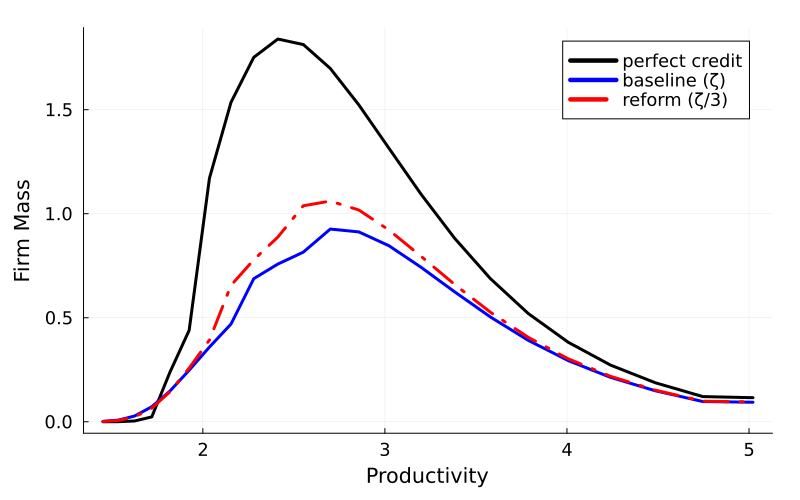
\includegraphics[width=\textwidth]{Plots/noise60_firm_mass_z3.png} \\
\scriptsize Firm mass across productivity states
\end{column}
\end{columns}

\end{frame}

%----------------------------------------------------------------------------------------
%	7 -- POLICY QUICK INTRO
%----------------------------------------------------------------------------------------
\begin{frame}[label=policy] \frametitle{Policy: The U.S., the EU and Lithuania \hfill \hyperlink{sources}{\beamergotobutton{Sources}}}

\textbf{What the U.S.\ does} \hfill \hyperlink{sbra_data}{\beamergotobutton{Subchapter V}}
\begin{itemize} \small
    \item Subchapter V (2020): cheaper, simplified reorganization for \textbf{small firms} (debt $<$ \$3M)
\end{itemize} \normalsize

\textbf{What the EU does}
\begin{itemize} \small
    \item Directive 2019/1023: preventive restructuring, cram-down, early warning for \textbf{all firms}
    \item Directive 2026/799: a simplified procedure for small firms is \textbf{left to Member States}
\end{itemize} \normalsize \vspace{1mm}

\begin{columns}[T,onlytextwidth]
\begin{column}{0.53\textwidth}
    \vspace{5mm} 
\textbf{What Lithuania does}
\begin{itemize} \small
    \item 2021: EU Restructuring Directive transposed
    \item One court procedure, built for large firms
    \item \textcolor{red}{\textbf{No simplified procedure for small firms}}
\end{itemize}
\end{column}
\begin{column}{0.44\textwidth}
\textbf{Practice} \\[1mm]
\footnotesize
\renewcommand{\arraystretch}{0.95}
\begin{tabular}{lcc}
\toprule
\textbf{Per year} & \textbf{Bankrupt.} & \textbf{Restruct.} \\
\midrule
Pre-COVID avg.  & $\sim$1,400 & $\sim$38 \\
2022            & 1,171 & 21 \\
2024            & 1,079 & $\sim$36 \\
\bottomrule
\end{tabular} \vspace{1mm}

\end{column}
\end{columns}

\end{frame}

%----------------------------------------------------------------------------------------
%	8 -- RECOMMENDATION 
%----------------------------------------------------------------------------------------


\begin{frame}[label=rec] \frametitle{Policy Recommendations \hfill \hyperlink{sbra_full}{\beamergotobutton{Full results}}}

The same reform, in three designs

\vspace{2mm}
\footnotesize
\centering
\renewcommand{\arraystretch}{0.9}
\begin{tabular}{lccc}
\toprule
 & \textbf{Uniform} & \textbf{Size-based} & \textbf{Uniform} \\
 & \textbf{Reform} & \textbf{Reform} & \textbf{+ weaker creditors} \\
\midrule
Firms' cost cut & 100\% & 35\% & 100\% \\
\midrule
Productivity $(Y/L)$ & \textcolor{primary}{+1.08\%} & \textcolor{primary}{+1.05\%} & \textcolor{red}{+0.32\%} \\
Pr.\ liquidation (pp) & $-$11.7 & $-$6.0 & $-$12.6 \\
CF reliance (pp)     & +7.7   & +0.3   & $-$5.9 \\
\bottomrule
\end{tabular}
\normalsize
\vspace{8mm}

\begin{columns}[T,onlytextwidth]
\begin{column}{0.48\textwidth}
\textbf{1. Target Smaller Firms}
\begin{itemize} \small
    \item Almost all gain comes from small and middle-market firms
    \item A single procedure designed for large companies misses this
\end{itemize}
\end{column}
\begin{column}{0.48\textwidth}
\textbf{2. Preserve creditor rights}
\begin{itemize} \small
    \item Cram-down lowers what lenders recover
    \item Lenders price in the weaker recovery
    \item Liquidations still fall, but most of the productivity gain is lost
\end{itemize}
\end{column}
\end{columns}

\end{frame}

%----------------------------------------------------------------------------------------
%	10 -- IMPLICATIONS FOR LITHUANIA
%----------------------------------------------------------------------------------------
\begin{frame}[label=implications] \frametitle{Conclusions and Implications for Lithuania}

High reorganization costs tpically push distressed firms into liquidation \vspace{-1.5mm}

\hspace{50mm} \textcolor{primary}{$\boldsymbol{\Downarrow}$} \vspace{-2mm}

Liquidation risk limits small firms' access to cash flow-based debt \normalsize \vspace{3mm}

\pause

Facilitating reorganization improves access to credit 
\begin{itemize} \small
    \item Cutting reorganization costs by two thirds lowers liquidation risk by $\sim$12 pp 
    \item Cash-flow credit becomes cheaper: small firms shift from collateral toward cash flows 
    \item More firms enter and survive, raising productivity by $\sim$1.1\%
\end{itemize} \normalsize \vspace{4mm}

\textbf{Policy recommendations for Lithuania}
\begin{itemize} \small
    \item Reduce reorganization costs without weakening creditor rights
    \item Adopt a simplified procedure for small firms {\footnotesize (option under Directive 2026/799)}
    \end{itemize}
 
\end{frame}


\appendix
\section{Appendix}

%------------------------------------------------
\begin{frame}[label=sources] \frametitle{Sources: Lithuania and the EU \hfill \hyperlink{motivation}{\beamergotobutton{Back}}}

\footnotesize
\begin{itemize}
    \item Bank of Lithuania and Competition Council (2021), SME financing study: rejections of very small firms 2018--19; recommendation of more efficient insolvency processes
    \item OECD (2026), \textit{Financing SMEs and Entrepreneurs 2026: Lithuania}: share of SMEs needing collateral (96\%, 2024)
    \item Bank of Lithuania, \textit{Financial Stability Review 2025}: enterprise survey; 97\% of firms cite insufficient collateral as a reason to use internal funds; corporate credit 16\% of GDP vs $\sim$31\% in the euro area
    \item Bank of Lithuania, \textit{Financial Stability Review 2026}, Box 1: two-thirds of corporate loans secured by real estate (EU median $\sim$40\%); unsecured loans only to large, strong firms
    \item bnt attorneys, INSOL Europe (Feb.\ 2023), summarising AVNT data: restructurings $\sim$2\% of insolvency proceedings since 2001, $\sim$11\% successful
    \item Eurofound, ERM legislation database: Law on Insolvency of Legal Entities (No XIII-2221)
    \item Directive (EU) 2019/1023; Directive (EU) 2026/799
\end{itemize}

\end{frame}

%------------------------------------------------
\begin{frame}[label=lithuania] \frametitle{Lithuania: A Modern Framework That Is Hardly Used \hfill \hyperlink{policy}{\beamergotobutton{Back}}}

\begin{columns}[T,onlytextwidth]
\begin{column}{0.53\textwidth}
\textbf{Law}
\begin{itemize} \small
    \item 2020: one insolvency law for bankruptcy and restructuring
    \item 2021: EU Restructuring Directive transposed
    \begin{itemize} \footnotesize
        \item restructuring once insolvency is \textit{likely}
        \item cross-class cram-down of creditors
        \item protection of new financing
        \item early warning via the Tax Inspectorate
    \end{itemize}
\end{itemize}
\end{column}
\begin{column}{0.44\textwidth}
\textbf{Practice} \\[1mm]
\footnotesize
\renewcommand{\arraystretch}{0.95}
\begin{tabular}{lcc}
\toprule
\textbf{Per year} & \textbf{Bankrupt.} & \textbf{Restruct.} \\
\midrule
Pre-COVID avg.  & $\sim$1,400 & $\sim$38 \\
2022            & 1,171 & 21 \\
2024            & 1,079 & $\sim$36 \\
\bottomrule
\end{tabular} \vspace{1mm}

\small Creditors recover $\sim$13\% in bankruptcy
\end{column}
\end{columns}
\vspace{3mm}

\normalsize
Commentators: a ``technical'' transposition
\begin{itemize} \small
    \item One court procedure, \textbf{designed for large companies}
    \item No simplified or out-of-court restructuring for micro and small firms
\end{itemize}

\src{Pre-COVID: bankruptcies 2001--19, restructurings 2008--20; recovery: 2015 audit. Counts mix openings and registrations.}

\end{frame}

%------------------------------------------------
\begin{frame}[label=ModelFit] \frametitle{Model Fit \hfill \hyperlink{Calibration}{\beamergotobutton{Calibration}}}

U.S.\ non-financial firms, 2010--2024 \footnotesize \textit{(Compustat, CapitalIQ, FJC IDB)} \normalsize
\begin{itemize} \small
    \item \textbf{Small:} liabilities below \$1bn (two thirds of firms); \textbf{large:} above \hfill \hyperlink{targets}{\beamergotobutton{Data}}
\end{itemize} \vspace{1mm}

\footnotesize
\begin{table}[h!]
\centering
\renewcommand{\arraystretch}{0.9}
\begin{tabular}{l|cc||cc}
& \multicolumn{2}{c||}{\textbf{All firms}} & \multicolumn{2}{c}{\textbf{By size} \scriptsize (Data -- \textcolor{primary}{Model})} \\
\toprule
Moment & Data & Model & Small firms & Large firms \\
\midrule
Liquidation prob.$^\dagger$  & 0.41 & \textcolor{primary}{0.42} & 0.50 -- \textcolor{primary}{0.50} & 0.24 -- \textcolor{primary}{0.24} \\
CF reliance$^\dagger$        & 0.52 & \textcolor{primary}{0.53} & 0.41 -- \textcolor{primary}{0.43} & 0.72 -- \textcolor{primary}{0.75} \\
\midrule
Debt to collateral          & 0.72 & \textcolor{primary}{0.72} & 0.66 -- \textcolor{primary}{0.65} & 0.85 -- \textcolor{primary}{0.96} \\
Interest rate (\%)          & 6.22 & \textcolor{primary}{6.29} & 6.87 -- \textcolor{primary}{7.10} & 5.05 -- \textcolor{primary}{4.49} \\
CF-based to total debt      & 0.82 & \textcolor{primary}{0.74} & 0.48 -- \textcolor{primary}{0.65} & 0.83 -- \textcolor{primary}{0.75} \\
\bottomrule
\end{tabular}
\end{table}
\vspace{-2mm}
\scriptsize $^\dagger$ Small--large gap targeted. Remaining size moments untargeted. \normalsize \vspace{2mm}

\begin{itemize} \small
    \item Matches liquidation risk and cash-flow borrowing of small and large firms
    \item Untargeted gaps in leverage and rates have the right sign, but are too wide
\end{itemize}

\end{frame}

%------------------------------------------------
\begin{frame}[label=slide_outline] \frametitle{Model Outline: Financial Intermediation \hfill \hyperlink{payoffs}{\beamergotobutton{Lender`s Payoffs}}}
\centering
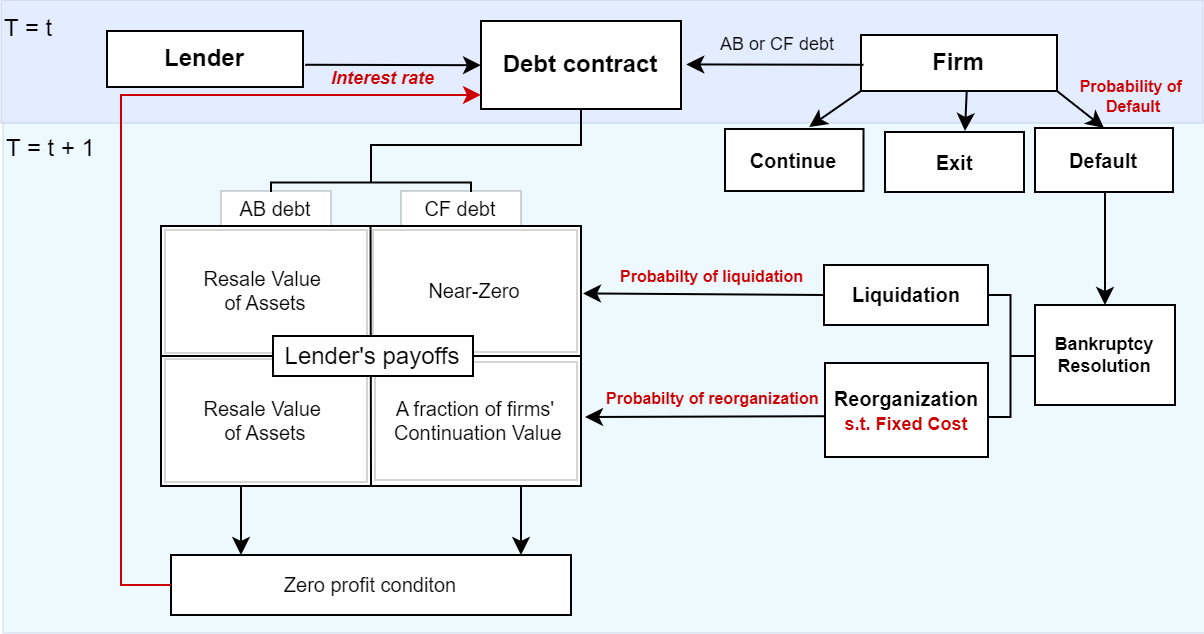
\includegraphics[width=0.92\textwidth]{Plots/min60_t7_fc.png}
\end{frame}

%------------------------------------------------
\begin{frame}[label=decomp] \frametitle{Decomposition of the Productivity Gain \hfill \hyperlink{aggregate}{\beamergotobutton{Back}}}

\[
\Delta\log\frac{Y}{N}
= \underbrace{\frac{\alpha}{1-\alpha}\,\Delta\log\frac{K}{Y}}_{\text{Capital Deepening}}
+ \frac{1}{1-\alpha}\Big[
\underbrace{(1-s)\Delta\log M}_{\text{Mass Effect}} +
\underbrace{(1-s)\Delta\log C}_{\text{Composition Effect}} +
\underbrace{\Delta\log\Omega}_{\text{Policy Residual}}\Big]
\]

\footnotesize
\begin{table}[h!]
\centering
\renewcommand{\arraystretch}{0.9}
\begin{tabular}{lcc}
\toprule
$\zeta \rightarrow \zeta/3$ & \textbf{Log points} & \textbf{Share} \\
\midrule
Output per worker, $Y/L$    & 1.07 & 1.00 \\
\midrule
Mass effect ($M$)           & 2.35 & 2.19 \\
Composition effect ($C$)    & $-$1.43 & $-$1.34 \\
Capital deepening ($K/Y$)   & 0.07 & 0.06 \\
Policy residual ($\Omega$)  & 0.08 & 0.08 \\
\bottomrule
\end{tabular}
\end{table}
\normalsize

\begin{itemize} \small
    \item More operating firms raise productivity; entrants are less productive on average, which partly offsets
    \item Capital per firm and firm policies change little
\end{itemize}

\end{frame}

%------------------------------------------------
\begin{frame}[label=allocation] \frametitle{Is Credit Better Allocated? \hfill \hyperlink{aggregate}{\beamergotobutton{Back}}}

$\zeta \rightarrow \zeta/3$; borrowing firms in the new steady state

\footnotesize
\begin{table}[h!]
\centering
\renewcommand{\arraystretch}{0.9}
\begin{tabular}{lccc}
\toprule
 & \textbf{Baseline} & \textbf{Reform} & \textbf{Change} \\
\midrule
Small firms' share of total debt              & 11.2\% & 12.2\% & +1.0 pp \\
Small firms' total debt                       & & & +9.3\% \\
Covariance of debt share and productivity     & 1.062 & 1.091 & +2.7\% \\
Dispersion of $\log(y/k)$, firm-weighted      & 0.303 & 0.291 & $-$4.1\% \\
Dispersion of $\log(y/k)$, capital-weighted   & 0.091 & 0.089 & $-$2.3\% \\
\bottomrule
\end{tabular}
\end{table}
\normalsize

\begin{itemize} \small
    \item Debt shifts slightly toward smaller and more productive firms
    \item The returns to capital become slightly more equal across firms
    \item These effects are small: the gain comes mainly from entry
\end{itemize}

\end{frame}

%------------------------------------------------
\begin{frame}[label=reformsize] \frametitle{Size of the Reform \hfill \hyperlink{effects}{\beamergotobutton{Back}}}

\footnotesize
\begin{table}[H]
\centering
\renewcommand{\arraystretch}{0.9}
\begin{tabular}{lcccc}
\toprule
 & $\zeta/2$ & $\zeta/3$ & $\zeta/10$ & \textbf{No credit frictions} \\
\midrule
Productivity $(Y/L)$         & +0.71\% & +1.08\% & +1.73\% & +9.0\% \\
No.\ of firms                & +8.0\% & +11.8\% & & \\
Pr.\ liquidation, small firms & 0.50 $\to$ 0.40 & 0.50 $\to$ 0.34 & & \\
CF reliance, small firms     & 0.43 $\to$ 0.50 & 0.43 $\to$ 0.53 & & \\
\bottomrule
\end{tabular}
\end{table}
\normalsize
\begin{itemize} \small
    \item Gains rise with the size of the cut, with diminishing returns
    \item ``No credit frictions'': firms can raise equity at no cost
\end{itemize}

\end{frame}

%------------------------------------------------
\begin{frame}[label=noise] \frametitle{Valuation Noise in Bankruptcy Courts \hfill \hyperlink{LiqReorg2}{\beamergotobutton{Liquidation rule}}}

Courts compare liquidation and reorganization values with a log-normal valuation error
\[
\Pr(\text{liquidation}) = \Phi\left( \frac{1}{\sigma_v} \ln \frac{\phi_a(1-\delta)k + \zeta}{(1-\phi_c)\,V_{cont}(x,\varepsilon)} \right)
\]
\begin{itemize} \small
    \item Without noise ($\sigma_v = 0$): large firms are almost never liquidated (data: 24\%)
    \item $\sigma_v = 1.48$ is calibrated to the gap between small and large firms' liquidation rates
\end{itemize} \vspace{3mm}

Noise damps the reform
\begin{itemize} \small
    \item Cheaper reorganization does not remove mistaken liquidations
    \item Suggests accurate valuation as a complement to cost cuts \textit{(not yet a model experiment)}
\end{itemize}

\end{frame}

%------------------------------------------------
\begin{frame}[label=Aggeffects] \frametitle{Alternative Models: Only One Debt Type \hfill \hyperlink{aggregate}{\beamergotobutton{Back}}}

Halving the fixed reorganization cost ($\zeta/2$), each model recalibrated

\small
\begin{table}[H]
    \centering
    \renewcommand{\arraystretch}{0.9}
    \begin{tabular}{lccc}
    & \textbf{Both debt types} & \textbf{Only asset-based} & \textbf{Only CF-based} \\
    \toprule
    Pr.\ liquidation (pp)  & $-$7.5 & $-$7.8 & $-$8.3 \\
    Productivity $(Y/L)$   & +0.71\% & 0\% & +0.85\% \\
    No.\ of firms          & +8.0\% & +1.7\% & +8.5\% \\
    Interest rate (pp)     & $-$0.38 & $-$0.04 & $-$0.72 \\
    \bottomrule
    \end{tabular}
\end{table}
\normalsize

\begin{itemize}
    \item Only asset-based debt: lower liquidation risk does not reach credit \\ \small (zero gain by construction: owners do not value reorganization)
    \item \normalsize Liquidation risk matters through cash flow-based lending
\end{itemize}

\end{frame}

%------------------------------------------------
\begin{frame}[label=sbra_full] \frametitle{Size-Based Reforms: Full Results \hfill \hyperlink{rec}{\beamergotobutton{Back}}}

\small
\begin{table}[H]
    \centering
    \renewcommand{\arraystretch}{0.9}
    \begin{tabular}{lccc}
    \textbf{Policy} & \textbf{Uniform} & \textbf{Size-based} & \textbf{+ weaker creditors}\\
    \toprule
    & $\zeta \rightarrow \zeta/3$ & $\zeta_{small} \rightarrow \zeta/3$ & $+\ \theta \rightarrow \tfrac{3}{4}\theta$\\
    \midrule
    Productivity $(Y/L)$       & +1.08\% & +1.04\% & +0.32\%\\
    No.\ of firms              & +11.8\% & +11.6\% & +5.0\%\\
    Capital int.\ $(K/L)$      & +1.25\% & +1.24\% & +0.49\%\\
    Pr.\ liquidation (pp)      & $-$11.7 & $-$10.5 & $-$11.4\\
    Debt to collateral (pp)    & +1.0 & +1.0 & $-$0.8\\
    Interest rate (pp)         & $-$0.58 & $-$0.58 & $-$0.52\\
    CF reliance (pp)           & +7.7 & +6.4 & $-$7.4\\
    CF-based to total debt (pp) & +3.2 & +0.5 & $-$23.1\\
    \bottomrule
    \end{tabular}
\end{table}
\normalsize
\scriptsize Noise60 calibration. Size-based: fixed cost cut for firms below the size cutoff only; uniform: for all firms. Third column adds a quarter off the lender's share of the reorganized firm.

\end{frame}

%------------------------------------------------
\begin{frame}[label=sbra_data] \frametitle{Sizing the Reform: U.S.\ Subchapter V \hfill \hyperlink{rec}{\beamergotobutton{Back}}}
V (2020): simplified reorganization for small businesses, debt limit \$3M (\$7.5M temporarily)
\begin{itemize} \small
    \item Faster plans, less disclosure, a trustee to aid negotiations
    \item Also weakens creditors: easier cram-down, relaxed absolute priority
\end{itemize} \vspace{2mm}

\textbf{Hotchkiss, Iverson, and Zheng, 2024:} plan confirmation rises by about \textbf{21 pp} (32.9\% $\to$ 54.9\%); unsecured creditors' recoveries not lower \vspace{2mm}

\textbf{Back-of-the-envelope}, with filing shares from the FJC database:
\[
\begin{aligned}
\text{2019 (pre-reform):}\;& 0.471 \times 0.329 = 0.155 \Rightarrow 84.5\% \text{ liquidation} \\
\text{2024 (post-reform):}\;& 0.520 \times 0.549 = 0.285 \Rightarrow 71.5\% \text{ liquidation}
\end{aligned}
\]
$\Rightarrow$ about 13 pp lower liquidation probability for eligible firms

\end{frame}

%------------------------------------------------
\begin{frame}[label=Calibration] \frametitle{Calibration \hfill \hyperlink{ModelFit}{\beamergotobutton{Back}}}

\footnotesize
\begin{table}[h!]
\centering
\renewcommand{\arraystretch}{0.85}
\begin{minipage}{0.48\textwidth}
\centering
\begin{tabular}{c|l|c}
\multicolumn{3}{l}{\textbf{External}} \\
\toprule
$\beta$ & Discount rate & 0.96 \\
$\alpha,\ \nu$ & Capital, labor elasticity & 0.28, 0.57 \\
$\delta$ & Depreciation & 0.065 \\
$\rho$ & Productivity persistence & 0.969 \\
$\sigma_\varepsilon$ & Productivity shock SD & 0.088 \\
$\phi_a$ & Resale value of assets & 0.425 \\
$\kappa$ & Unsecured discount & 0.1 \\
\bottomrule
\end{tabular}
\end{minipage}
\hfill
\begin{minipage}{0.48\textwidth}
\centering
\begin{tabular}{c|l|c}
\multicolumn{3}{l}{\textbf{Internal}} \\
\toprule
$\zeta$ & Fixed reorg.\ cost & 1199 \\
$\phi_c$ & Variable reorg.\ cost & 0.07 \\
$\theta$ & Lender's share in reorg. & 0.22 \\
$\sigma_v$ & Valuation noise & 1.48 \\
$P_x$ & Exogenous distress prob. & 0.005 \\
$c$ & Fixed operating cost & 40.7 \\
$c_e$ & Entry cost (wage $=1$) & 477.5 \\
\bottomrule
\end{tabular}
\end{minipage}
\end{table}
\normalsize

\begin{itemize} \small
    \item Targets: five aggregate moments + small--large gaps in liquidation and CF reliance
    \item Decreasing returns $\alpha + \nu = 0.85$
\end{itemize}

\end{frame}

%------------------------------------------------
\begin{frame}[label=targets] \frametitle{Data and Size Classes \hfill \hyperlink{ModelFit}{\beamergotobutton{Back}}}

Combination of CapitalIQ, Compustat, and FJC's IDB data, 2010--2024 \vspace{3mm}
\begin{itemize} \small
    \item Moments weighted by the Compustat firm distribution
    \item Micro firms ($<$100k assets) excluded
    \item \textbf{Small:} total liabilities below \$1bn (67\% of firms); \textbf{large:} above
\end{itemize} \vspace{3mm}

Why U.S.\ data
\begin{itemize} \small
    \item Only source linking debt contracts (asset vs cash flow-based) to bankruptcy outcomes by size
    \item A Lithuanian calibration would need credit register and insolvency-court data
\end{itemize}

\end{frame}

%------------------------------------------------
\begin{frame}[label=FCreorg] \frametitle{Fixed Costs of Reorganization \hfill \hyperlink{evidence}{\beamergotobutton{Back}}}

Reorganization: lengthy negotiation between debtors and creditors
\begin{itemize} \small
    \item Large legal, administrative and time (direct and indirect) costs
    \item Often involves the costs of replacing original management
\end{itemize} \normalsize \vspace{8mm}

\textbf{Fixed cost} of reorganization - \footnotesize \textit{Wang, 2022, Bris et al. 2006, LoPucki and Doherty, 2011}
\begin{itemize} \small
    \item Smaller firms face higher reorganization costs per dollar of assets
    \item Smaller firms take longer to reorganize per dollar of assets
\end{itemize} \normalsize

\end{frame}

%------------------------------------------------
\begin{frame}[label=LiqReorg2] \frametitle{Liquidation Probability \hfill \hyperlink{ModelSummary}{\beamergotobutton{Back}}}

Bankruptcy courts maximize the \textit{joint value} retained after bankruptcy,
\begin{equation*}
    \max \{ \underbrace{\phi_a (1-\delta) k}_{\textcolor{primary}{\text{Value in Liquidation}}}   ; \ \underbrace{(1-\phi_c) V_{cont}(x,\varepsilon)- \zeta}_{\textcolor{primary}{\text{Value in Reorganization}}}   \}
\end{equation*}
\begin{itemize} \small
    \item The court observes the reorganization value with log-normal error, s.d.\ $\sigma_v$ \hfill \hyperlink{noise}{\beamergotobutton{Noise}}
\end{itemize} \vspace{2mm}

Ex-ante probability of liquidation in default:
\begin{equation*}
    \gamma(k', b', \varepsilon) = \E \left[ \Phi\left( \frac{1}{\sigma_v} \ln \frac{\phi_a(1-\delta)k' + \zeta}{(1-\phi_c) V_{cont}(x',\varepsilon')} \right) \Big| \ \chi_d = 1 \right]
\end{equation*}
\textbf{Fixed costs} $\zeta$ $\Rightarrow$ liquidation probability decreases with firm size

\end{frame}

%------------------------------------------------
\begin{frame}[label=payoffs] \frametitle{The Lender's In-Default Payoffs \hfill \hyperlink{slide_outline}{\beamergotobutton{Back}}}

\begin{table}[h!]
\centering
\resizebox{0.55\textwidth}{!}{
\begin{tabular}{l|cc}
& Asset-based debt & CF-based debt  \\
\midrule
Liquidation & $\phi_a (1-\delta) k$ &$\kappa\phi_a (1-\delta) k$ \\
Reorganization & $\phi_a (1-\delta) k$ &$\theta V_{cont}(x, \varepsilon)$ \\
\bottomrule
\end{tabular}
}
\end{table}

Under liquidation, the lender recovers
$$   \Pi_{l}(a) =  \min \{b, \ \ (1-\tau) \underbrace{\phi_a (1-\delta) k}_{\textcolor{primary}{\text{AB, Liq}}} + \tau \underbrace{\kappa \phi_a  (1-\delta) k}_{\textcolor{primary}{\text{CF, Liq}}} \} $$
Under reorganization, the lender negotiates the transfer:
$$ \Pi_{r}(a,\varepsilon) = \min \{b, \ \  (1-\tau) \underbrace{\phi_a (1-\delta) k}_{\textcolor{primary}{\text{AB, Reorg}}} +\tau \underbrace{\theta V_{cont} (x, \varepsilon)}_{\textcolor{primary}{\text{CF, Reorg}}} \} $$

\end{frame}

%------------------------------------------------
\begin{frame}[label=Qfull] \frametitle{The Inverse Interest Rate \hfill \hyperlink{ModelSummary}{\beamergotobutton{Back}}}

The lender considers: \small
\begin{itemize}\setlength\itemsep{0em}
    \item Probability of default, $P_D(a', \varepsilon)$
    \item Probability of liquidation in default $\gamma(k',b', \varepsilon)$
    \item Expected payoffs under liquidation and reorganization,  $\Pi_{l}(a')$, $\Pi_{r}(a', \varepsilon)$
\end{itemize} \normalsize

Inverse interest rate ($q$) defined by the zero profit condition:
\begin{equation*}
    \begin{split}
        & q(a', \varepsilon)b' = q_0 [ \left(1-P_D(a', \varepsilon)\right)b' +  \\
        & \qquad \qquad \underbrace{P_D(a', \varepsilon)}_{\textcolor{primary}{\text{Pr(Default)}}} \underbrace{\gamma(a', \varepsilon)}_{\textcolor{primary}{\text{\quad Pr(Liq.) \quad }}} \underbrace{\Pi_{l}(a')}_{\textcolor{primary}{\text{Recovery Liq. }}} + \\
        & \qquad  \qquad \underbrace{P_D(a', \varepsilon)}_{\textcolor{primary}{\text{Pr(Default)}}}  (\underbrace{1-\gamma(a', \varepsilon)}_{\textcolor{primary}{\text{Pr(Reorg.) }}})\ E_{\varepsilon' | \varepsilon} [ \underbrace{\Pi_{r}(a', \varepsilon')}_{\textcolor{primary}{\text{Recovery Reorg. }}} |\chi_r = 1 ] ]
    \end{split}
\end{equation*}

Continuing firms choose $(k',b',\tau')$ to maximize $V_{cont}(x,\varepsilon)$ s.t.\ $q(k',b',\tau', \varepsilon)$

\end{frame}

%------------------------------------------------
\begin{frame}[label = LandM] \frametitle{Cash Flow-Based and Asset-Based Lending \hfill \hyperlink{motivation}{\beamergotobutton{Back}}}

Asset-based lending:
\begin{itemize} \small
\item Secured against borrowers' physical assets
\item \textbf{Creditors in-default payoffs}: value of physical collateral
\end{itemize} \normalsize \vspace{4mm}

Cash flow-based lending:
\begin{itemize} \small
\item No \textit{specific} assets pledged as collateral
\item Secured against the entire corporate entity, or unsecured
\item \textbf{Creditors in-default payoffs}: expected future cash flows
\end{itemize} \normalsize  \vspace{4mm}

Lian and Ma (2021): 80\% of U.S.\ corporate debt is backed by future cash flows

\end{frame}

\end{document}
